\subsubsection{Incremento 7}
\textit{\textbf{Periodo}: dal 2021-03-19 al 2021-03-25}

\myparagraph{Obiettivi}
Gli obiettivi definiti per questo incremento sono i seguenti:
\begin{itemize}
\item implementazione autenticazione della visualizzazione dei prodotti (pagine di listino) e della dashboard venditore;
\item incremento della documentazione.
\end{itemize}

\myparagraph{Attività}
Per raggiungere gli obiettivi, vengono svolte le seguenti attività:
\begin{itemize}

\item \textbf{codifica e pianificazione}:
\begin{itemize}
\item implementazione UC16 - Ricerca nel catalogo digitale;
\item implementazione UC17 - Accesso ad una pagina della categoria;
\item implementazione UC18 - Visualizzazione dei prodotti;
\item implementazione UC19 - Selezione dei prodotti;
\item implementazione UC21 - Filtraggio dei prodotti;
\item implementazione UC23 - Visualizzazione del prodotto;
\item implementazione UC26 - Accesso alla merchant dashboard;
\item implementazione UC27 - Inserimento prodotto;
\item implementazione UC28 - Visualizzazione lista prodotti;
\item implementazione UC29 - Modifica prodotto;
\item implementazione UC30 - Rimozione prodotto;
\item implementazione UC31 - Visualizzazione lista categorie;
\item implementazione UC31 - Inserimento categoria;
\item implementazione UC32 - Rimozione categoria;
\item implementazione UC35 - Visualizzazione collegamenti a sistemi di gestione;
\item creazione diagrammi UML inerenti.

\end{itemize}

\item \textbf{ampliamento documentazione e verifiche}:
\begin{itemize}
\item incremento del \textit{\MU{}} per i casi d'uso implementati;
\item incremento del \textit{\MM{}} per i casi d'uso implementati;
\item incremento dell'\textit{Allegato tecnico}\ped{G} per i casi d'uso implementati;
\item incremento del \Glossariov{3.0.0};
\item rilevazione e registrazione di metriche, esiti di verifica e obiettivi di qualità;
\item aggiornamento dei rischi rilevati;
\item calcolo e registrazione del consuntivo di periodo.
\end{itemize}

\end{itemize}
\myparagraph{Diagramma di Gantt}
\begin{figure}[H]
\centering

\centerline{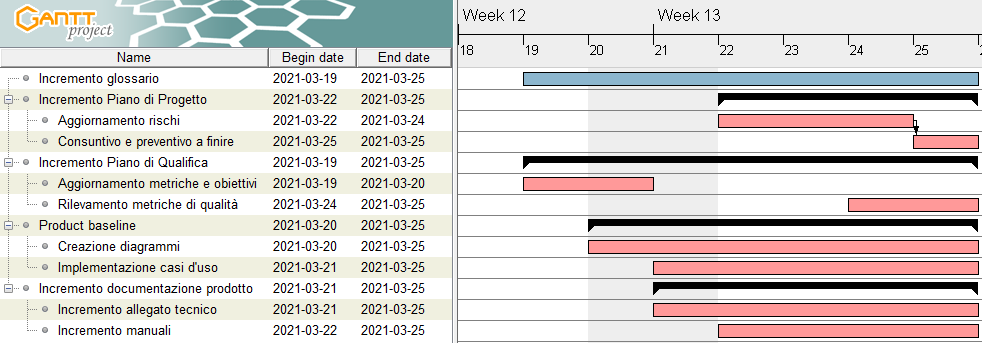
\includegraphics[scale=0.6]{res/Pianificazione/Fasi/CodificaIncrementi/ganttIncremento7}}
\caption{Diagramma di Gantt per l'incremento 7}
\end{figure}